% !TEX program = xelatex
%\documentclass[11pt,letterpaper]{article}
%\usepackage{beamerarticle}
\documentclass[notes=hide]{beamer}
%\documentclass[notes=show]{beamer}
%\documentclass[handout]{beamer}

\usepackage{newtxtext}
\usepackage{bucolors}
\usepackage{analchem}
\usepackage{lecture}
\usepackage{pdfpages}
\usepackage{ccicons}
\usepackage{multicol}

\graphicspath{{./Figures/}}

\title{Introduction to Analytical Chemistry}
\author{D.A.\ McCurry}
\institute[Bloomsburg University] % (optional)
{Department of Chemistry and Biochemistry\\
  Bloomsburg University}
\date{Fall 2021}

\begin{document}

%\mode<presentation>{
%
%\begin{frame}<handout:0>{Welcome to Analytical Chemistry I!}
%	\centering
%
%	\includegraphics[width=\linewidth]{lasvegas.png}
%\end{frame}
%}

\maketitle

\begin{frame}
	\section{What is Analytical Chemistry?}
\end{frame}

\mode<article>{%
	Analytical chemistry deals with the
	identification and separation of materials \alert{and} the
	determination of its relative amount.

	\begin{center}
		\sffamily
		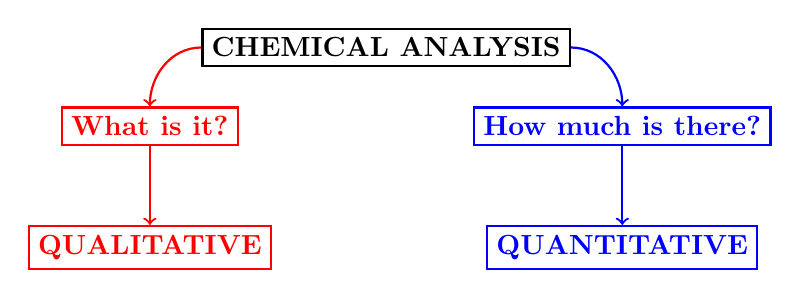
\begin{tikzpicture}
			\node[draw,thick](title) at (0,0) {\bfseries CHEMICAL
				ANALYSIS};
				\node[draw,thick,red](qual) at (-3,-1)
				{\bfseries What is it?};
				\draw[->,thick,red] (title.west) to
				[in=90,out=180] (qual.north);
				\node[draw,thick,blue](quant) at (3,-1)
				{\bfseries How much is there?};
				\draw[->,thick,blue] (title.east) to
				[in=90,out=0] (quant.north);
				\draw[->,thick,red] (qual.south) to ++(0,-1)
				node[below,draw,thick,red]{\bfseries
				QUALITATIVE};
				\draw[->,thick,blue] (quant.south) to ++(0,-1)
				node[below,draw,thick,blue]{\bfseries
				QUANTITATIVE}; 
		\end{tikzpicture}
	\end{center}
}

\begin{frame}{Why is analytical chemistry important?}
	\mode<presentation>{%
		\centering
		\includegraphics[width=\textwidth,trim={0.75in 4.25in 0.75in 1.5in},clip]{COVIDsensor.pdf}
	}
	\mode<article>{\textit{Anal. Chem.} \textbf{2020}, 92, 7226-7231}
\end{frame}

\begin{frame}{Steps in Chemical Analysis}
	\begin{center}
		\includegraphics[scale=0.7]{AnalyticalProcess.png}
	\end{center}
\end{frame}

\begin{frame}
	\section{A little review\ldots}
	\begin{center}
	\parbox{0.5\linewidth}{
	\begin{itemize}
		\item Units
		\item Concentration
		\item Exponents
		\item Dilutions
	\end{itemize}
}
\end{center}
\end{frame}

\begin{frame}{Units}
	\begin{itemize}
		\item Units are \emph{very} important in analytical chemistry!

		\item Common units and terms:
	\begin{center}
	\begin{tabular} {l l c c c}
		length: & meter & \si{\meter} \\
		mass: & kilogram & \si{\kilo\gram} \\
		time: & second & \si{\second} \\
		electric current: & ampere & \si{\ampere} \\
		temperature: & kelvin & \si{\kelvin} \\
		pressure: & pascal & \si{\pascal} & \emph{or} &
			\si{\newton\per\meter\squared} \\
	\end{tabular}
	\end{center}

	\begin{block}{Syst\`{e}me International d'Unit\'{e}s (SI units)}
		see Chapter 2, Section 1 in the text
	\end{block}
	\end{itemize}
\end{frame}

\begin{frame}[allowframebreaks]{Improper units can be catastrophic!}
	\begin{center}
		\includegraphics[scale=0.7]{Gimli_glider.JPG}
	\end{center}
	
	\footnotesize By Source, Fair use,
	https://en.wikipedia.org/w/index.php?curid=18952968

	\framebreak

	\begin{center}
		\includegraphics[scale=0.4]{MarsOrbiter.pdf}
	\end{center}
\end{frame}

\begin{frame}{Concentrations}
	The amount of \alert{solute} dissolved in a specific amount of
	\alert{solution} or \alert{solvent}.
	\begin{align*}
		\intertext{Some common examples you have probably seen before:}
		\text{molarity (\si{\Molar})} &=
		\dfrac{\text{\si{\mole}~solute}} {\text{\si{\liter}~solution}}
		\\
		\text{molality (\si{\molal})} &=
		\dfrac{\text{\si{\mole}~solute}}
		{\text{\si{\kilo\gram}~solvent}}
		\visible<2>{
		\intertext{And some you might not have:}
		\text{formality (\si{\formal})} &=
		\dfrac{\text{\si{\mole}~\alert{ionic~compounds}}}
		{\text{\si{\liter}~solution}} \\
		\text{normality (\si{\normal})} &= \dfrac{\text{reactive
		\alert{equivalents}}}{\text{\si{\liter}~solution}}
		}
	\end{align*}
\end{frame}

\begin{frame}<presentation>{Why bother with formality?}
	\begin{center}
		\includegraphics[width=\linewidth]{formality-scale.png}
	\end{center}
\end{frame}

\mode<article>{%
		\begin{itemize}
		\item Long answer: it is more reflective of the actual
			concentration of the species present in solution
			\begin{itemize}
				\item Strong electrolytes dissociate completely
					in solution:
					\begin{reaction*}
						!(\SI{1}{\formal})(NaCl) ->[ H2O
						] !(\SI{1}{\Molar})( Na+ ) +
						!(\SI{1}{\Molar})( Cl- )
					\end{reaction*}
				\item Weak electrolytes do not dissociate
					completely in solution:
					\begin{reaction*}
						!(\SI{1}{\formal})( HF ) <=>[ H2O ]
						!(\SI{<1}{\Molar})( H+ ) +
						!(\SI{<1}{\Molar})( F- )
					\end{reaction*}
			\end{itemize}
		\item Short answer: most often we don't --- it is widely understood that molarity $\equiv$ formality.
	\end{itemize}
}

\begin{frame}<presentation>{Why bother with normality?}
	\begin{center}
		\includegraphics[scale=0.5]{normality.jpg}
	\end{center}
\end{frame}

\mode<article>{%
	\begin{itemize}
		\item For some reactions, it may be more convenient to consider
			the \alert{reactive equivalents} offered by a reactant
		\item In particular, \alert{acid-base titrations} can be a bit
			simpler to think of in terms of normality

			\begin{center}
				\ch{H2SO4 + 2 NaOH -> Na2SO4 + 2 H2O}
			\end{center}

			\emph{Both} \ch{H+} in \ch{H2SO4} will react with
			\ch{OH-} to produce 2 \emph{equivalents} of \ch{H2O}
			\begin{align*}
				\therefore \SI{1}{\Molar}~\ch{H2SO4} &=
				\SI{2}{\normal}~\ch{H2SO4}
			\end{align*}
	\end{itemize}
}


\begin{frame}[t]{Conversions}
	A concentrated HF solution is \SI{48.1}{\percent} by weight \ch{HF} and
	has a density of \SI{1.15}{\gram\per\milli\liter}. What are the formal
	and molal concentrations of \ch{HF}?
\end{frame}

\mode<article>{%
	\begin{enumerate}
		\item Assume \SI{100.0}{\gram}~solution $\therefore$
			\SI{48.1}{\gram}~HF and \SI{51.9}{\gram}~\ch{H2O}
		\item Calculate moles HF: \SI{2.393}{\mole}~\ch{HF}
		\item This is enough to provide molality:
			\begin{align*}
				\dfrac{\SI{2.393}{\mole}~\ch{HF}}
				{\SI{0.0519}{\kilo\gram}~\text{solvent}}
				= \SI{46.1}{\molal}~\ch{HF}
			\end{align*}
		\item Use density to find volume of solution:
			\begin{align*}
				\SI{100.0}{\gram}~\text{solution} \times
				\dfrac{\SI{0.001}{\liter}}{\SI{1.15}{\gram}} =
				\SI{0.08696}{\liter}
			\end{align*}
		\item Calculate formality:
			\begin{align*}
				\dfrac{\SI{2.393}{\mole}}{\SI{0.08696}{\liter}}
				= \SI{27.5}{\formal}~\ch{HF}
			\end{align*}
	\end{enumerate}
}

\begin{frame}[t]{Exponent Removal}
	The concentration of barium ion in a produced water sample was found to
	be \SI{2.51e-7}{\Molar}.

	\begin{itemize}[<+->]
		\item Prefixes (kilo, milli, centi, \ldots)
			\only<.>{%
				\begin{align*}
					\SI{2.51e-7}{\Molar} =
					\dfrac{\SI{2.51e-7}{\mole}}{\si{\liter}}
					\times
					\dfrac{\SI{e6}{\micro\mole}}{\SI{1}{\mole}} =
					\SI{0.251}{\micro\Molar}
				\end{align*}
			}
		\item p-function: $\p{\ch{X}} = -\log [\ch{X}]$
			\only<.>{%
				\begin{align*}
					\p{\ch{Ba}} = -\log(\num{2.51e-7}) = 6.600
				\end{align*}
			}
		\item parts-per-concentrations (ppm, ppb, ppt, \ldots)
			\only<.->{%
				\begin{align*}
					\SI{2.51e-7}{\Molar} \times
					\SI{137327}{\milli\gram\per\mole}~\ch{Ba} &=
					\SI{0.0344}{\milli\gram\per\liter}~\ch{Ba^{2+}}
					\\
					&= \SI{0.0344}{ppm}\footnotemark[1]~\ch{Ba^{2+}} \\
					&= \SI{34.4}{ppb}\footnotemark[1]~\ch{Ba^{2+}}
				\end{align*}

				\bigskip
				\footnotetext[1]{Only in water ($d = \SI{1.00}{\gram\per\milli\liter}$), ppm = mg/L;
			ppb = \si{\micro\gram}/L;  ppt = ng/L.}
			}
	\end{itemize}

	\pause[\thebeamerpauses]

	\mode<presentation>{\vspace{-3em}}
	\begin{center}
		\bfseries
		Why is \SI{1}{\milli\gram\per\liter} = \SI{1}{ppm}?
	\end{center}
\end{frame}

\mode<article>{%
	\begin{align*}
		\text{ppm} &= \dfrac{\SI{1}{part}}{\SI[inter-unit-product={ }]{1}{million~parts}} =
			\dfrac{\SI{1}{part}}{\SI{e6}{parts}} \\
			\shortintertext{}
		d_{\ch{H2O}} &= \dfrac{\SI{1}{\gram}}{\SI{1}{\milli\liter}} =
		\dfrac{\SI{1}{\gram}}{\SI{e-3}{\liter}} \times
		\dfrac{\SI{1}{\milli\gram}}{\SI{0.001}{\gram}} =
		\dfrac{\SI{1}{\milli\gram}}{\SI{e-6}{\liter}} =
		\SI{e6}{\milli\gram\per\liter}\\
	\end{align*}

	$\therefore$ in \SI{1}{\liter}~\ch{H2O}, we have
\SI{e6}{\milli\gram}~\ch{H2O}, or ``\SI[inter-unit-product={ }]{1}{million~parts}''.}

\begin{frame}[t]{Dilutions}
	\begin{align*}
		M_\text{conc} V_\text{conc} = M_\text{dil} V_\text{dil}
	\end{align*}

	How would you prepare a liter of \SI{0.200}{\formal}~\ch{HCl} from
	\SI{11.8}{\formal} stock?

	\pause

	\mode<presentation>{\vskip0pt plus 1filll}

	\mode<article>{%
	\begin{align*}
		(\SI{11.8}{\formal})(V_\text{conc}) &=
		(\SI{0.200}{\formal})(\SI{1.00}{\liter}) \\
		V_\text{conc} &=
		\dfrac{(\SI{0.200}{\formal})(\SI{1.00}{\liter})}{\SI{11.8}{\formal}} \\
		V_\text{conc} &= \SI{17.0}{\milli\liter}
	\end{align*}
	}

	\begin{block}{Lab Technique:}
		Transfer $V_\text{conc}$ concentrated \ch{HCl} to a
		\SI{1.00}{\liter} volumetric flask and dilute to volume. Shake
		well at intermediate and final volume.
	\end{block}
\end{frame}

\begin{frame}[t]{Problem}
	A pesticide (\SI{408.8}{amu}) is extracted from a \SI{1.000}{\liter}
	ground water sample into \SI{25.00}{\milli\liter} of hexane. GC
	analysis indicates the latter solution contains \SI{52.1}{ppb}
	pesticide. What is the molar concentration in the original ground
	water?

	\pause

	\begin{center}
		(The density of hexane is \SI{0.6548}{\gram\per\milli\liter})
	\end{center}
\end{frame}

\mode<article>{%
	\begin{align*}
		\si{ppb} &= \dfrac{\text{mass of substance}}{\text{mass of sample}} \times \num{e9} \\
	\text{mass of sample}  &= \SI{25.00}{\milli\liter}~\text{hexane} \times \dfrac{\SI{0.6548}{\gram}}{\SI{1}{\milli\liter}} = \SI{16.37}{\gram}~\text{hexane} \\
\SI{52.1}{ppb} &= \dfrac{x}{\SI{16.37}{\gram}} \times \num{e9} \therefore x = \SI{8.529e-7}{\gram}~\text{pesticide} \\
		& \SI{8.529e-7}{\gram}~\text{pesticide} \times \dfrac{\SI{1}{\mole}}{\SI{408.8}{\gram}} = \SI{2.086e-9}{\mole} \\
		& \therefore \fbox{\SI{2.09e-9}{\Molar} or \SI{2.09}{\nano\Molar}}
	\end{align*}
}

\begin{frame}<1-4>[label=vocab]
	\section{The Vocabulary of Analytical Chemistry}
	\begin{center}
	\begin{multicols}{2}
		\begin{itemize}[<alert@+(1)>]
			\item Analyte vs Matrix
			\item Signal and Calibration
			\item Accuracy vs Precision
			\item Sensitivity vs Selectivity
			\item Robust vs Rugged
			\item Reagent vs Method vs Field~Blank
			\item Technique vs Method vs Procedure vs Protocol
			\item Validation
			\item Sampling
		\end{itemize}
	\end{multicols}
	\end{center}
\end{frame}

\mode<article>{%
	\begin{itemize}
		\item The analyte is what we're trying to measure. Ideally, it
			provides some type of signal that is proportional to its
			concentration or amount:
			\begin{equation*}
				S_{\ch{A}} = k_{\ch{A}}n_{\ch{A}}
			\end{equation*}
		\item In order to match up that concentration, we often create a
			calibration curve of known concentrations or amounts.
			\begin{equation*}
				y = mx+b
			\end{equation*}
		\item When we run an analysis, we often want it to be
			\emph{accurate}. Furthermore, when we run some over and
			over again, we expect to get the same results!
		\item 
	\end{itemize}
}

\begin{frame}[c]
	\frametitle{Accuracy vs Precision}

	\begin{center}
		\includegraphics[scale=0.85]{dartboard.png}
	\end{center}
\end{frame}

\againframe<5|handout:0>{vocab}

\begin{frame}{Specificity/Selectivity}
	\begin{columns}
		\column{0.5\linewidth}
	The ability of an analytical method to distinguish analyte from the
	sample matrix.

		\column{0.5\linewidth}
	\begin{center}
		\includegraphics[scale=0.2]{specificity.jpg}
	\end{center}
	\end{columns}

	\begin{exampleblock}{Cross-reactivity}
		\begin{columns}
			\column{0.5\linewidth}
			Often, analytical biochemical analyses 
			require a demonstration of \alert{specific
			binding} with the analyte.

			\column{0.4\linewidth}
			\centering
			\includegraphics[width=0.9\linewidth]{cross-reactivity.jpg}
		\end{columns}

			\tiny Sloan, C. D. K.; Marty, M. T.; Sligar, S. G.;
			Bailey, R. C. \textit{Anal. Chem.} \textbf{2013}, 85
			(5), 2970–2976.
	\end{exampleblock}
\end{frame}

\begin{frame}<presentation|handout:0|article:0>
	\begin{center}
		\includegraphics[width=0.9\linewidth]{cross-reactivity.jpg}
	\end{center}
\end{frame}

\againframe<6-8|handout:0>{vocab}

\begin{frame}
	\frametitle{Technique vs Method vs Procedure vs Protocol}
	\begin{center}
		\begin{tikzpicture}
			\tikzstyle{box}=[draw,thick,align =
			center,fill=bugold!50!white];
			\tikzstyle{arrow}=[->,thick];
			\node at (0,0) {Techniques};
			\node at (0,-2) {Methods};
			\node at (0,-4) {Procedures};
			\node at (0,-6) {Protocols};
			\node[box](GFAAS) at (5.5,0) {Graphite Furnace Atomic
				Absorption Spectroscopy \\ (GFAAS)};
			\node[box](soil) at (2.5,-2) {Pb in Soil};
			\node[box](water) at (5.5,-2) {Pb in Water};
			\node[box](blood) at (8.5,-2) {Pb in Blood};
			\node[box](APHA) at (4,-4) {APHA};
			\node[box](ASTM) at (7,-4) {ASTM};
			\node[box](EPA) at (5.5,-6) {EPA};
			\draw[arrow](GFAAS) -- (soil);
			\draw[arrow](GFAAS) -- (water);
			\draw[arrow](GFAAS) -- (blood);
			\draw[arrow](water) -- (APHA);
			\draw[arrow](water) -- (ASTM);
			\draw[arrow](water) -- (EPA);
		\end{tikzpicture}
	\end{center}
\end{frame}

\againframe<9|handout:0>{vocab}

\begin{frame}{Method Validation}
	The process of proving that an analytical method is acceptable for its
	intended purpose.

	\begin{center}
		\textbf{The Theranos Minilab}

		\vspace{1em}

		\includegraphics[width=0.6\linewidth]{theranos-minilab.jpg}
	\end{center}

	\footnotetext{\href{https://web.archive.org/web/20170627134226/https://www.theranos.com/
	}{\tiny https://web.archive.org/web/20170627134226/https://www.theranos.com/ (accessed Sep 10,
	2018)}}
\end{frame}

\againframe<10|handout:0>{vocab}

\begin{frame}{Constructing a Representative Sample}
	\begin{itemize}
		\item Chemical analysis is meaningless if we cannot demonstrate
			that the sample is \alert{representative} of the
			population.
		\item What factors influence the validity of the data?
	\end{itemize}

	\begin{center}
		\includegraphics[width=\linewidth]{box0-1.png}
	\end{center}
\end{frame}

\begin{frame}<presentation>
	\begin{center}
		\includegraphics[width=0.8\linewidth]{RadNet-US.png}
	\end{center}
	\let\thefootnote\relax\footnotetext{\url{https://www.epa.gov/radnet/near-real-time-and-laboratory-data-state}}
\end{frame}

\begin{frame}<presentation>
	\centering
	\includegraphics[width=0.95\linewidth,page=1]{CostNews2012Nov.pdf}
\end{frame}

\end{document}
		
